\documentclass[11pt]{beamer}
\usepackage{amsmath}
\usepackage{amsfonts}
\usepackage{amsthm}
\usepackage{graphicx}
\usepackage{listings}
\usepackage{multimedia}


\usetheme{Dresden}
\usecolortheme{seahorse}


%%theorems
\theoremstyle{plain}
\newtheorem{thm}{Theorem}[section]
\newtheorem{lem}[thm]{Lemma}

\theoremstyle{definition}
\newtheorem{defn}[thm]{Definition}
\newtheorem{prob}[thm]{Problem}


\theoremstyle{remark}
\newtheorem{rmk}[thm]{Remark}
\newtheorem{ex}[thm]{Example}

%%definitions
\newcommand{\of}[1]{\!\left(#1\right)}


\newcommand{\domain}{\Omega}
\newcommand{\boundary}{\Gamma}
\newcommand{\flow}{\vec v}
\newcommand{\refeq}[1]{(\ref{eq:#1})}

\lstset{
           basicstyle=\fontsize{7}{3}\ttfamily,
           keywordstyle=\color{blue}\ttfamily,
           stringstyle=\color{red}\ttfamily,
           commentstyle=\color{green}\ttfamily,
           breaklines=true,
           numbers=left,  
		   numbersep=5pt,
		   keepspaces=true,
          }


\title{\textbf{The Trace Finite Element Method for PDEs on Surfaces}}
\author{T. Jawecki, M. Wess}
\date{\today}
\begin{document}
\frame{\titlepage}

\begin{frame}
	\frametitle{Table of Contents}
	\tableofcontents
\end{frame}

%%%%%%%%%%%%%%section1
\section{Derivation of the model problem}
\begin{frame}
    \frametitle{General setting}
    \begin{columns}[T]
    	\begin{column}{0.5\textwidth}
			\begin{figure}[p]
				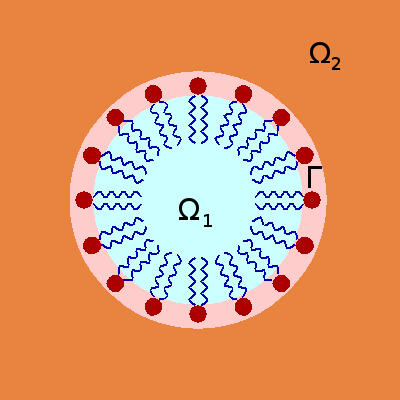
\includegraphics[width=0.7\textwidth]{surfactant3.png}
			\end{figure}
		\end{column}
		\begin{column}{0.5\textwidth}
			\begin{itemize}
				\pause
				\item{two fluids $\domain_1,\domain_2$ contained in an open domain, seperated by $\boundary$}
				\pause
				\item{given flux $\flow$}
				\pause
				\item{concentration $c$ of surfactant agent on $\boundary$}
			\end{itemize}
		\end{column}
	\end{columns}
	\pause
	\begin{prob}
		For given initial data $c_0$, find a model for the evolution of $c$.
	\end{prob}
\end{frame}
\begin{frame}
	\frametitle{Surface gradient and divergence}
		\begin{itemize}[<+->]
			\item{Smooth hypersurface $\boundary\subseteq\mathbb{R}^d$, outward normal $\vec n_\boundary$}
			\item{$C^1$-functions $f:\boundary\to\mathbb{R}$, $\vec g:\boundary\to\mathbb{R}^d$}
		\end{itemize}
	\only<3->{	
	\begin{defn}
		\begin{align*}
			\nabla_\boundary f&:=P\nabla f:=\left(I-\vec n_\boundary \vec n_\boundary^T\right)\!\nabla f\\
			\textrm{div}_\boundary \vec g&:=\nabla_\boundary\cdot \vec g:=\sum_{i=1}^d\sum_{j=1}^dp_{ij}\frac{\partial g_i}{\partial x_j}
		\end{align*}
	\end{defn}}
\end{frame}




\begin{frame}
    \frametitle{Reynolds transport theorem on an interface}

	\begin{thm}[Reynold's transport theorem on an interface]
	The rate of change for a smooth function $f(x,t)$ on $W\of{t}\subseteq \boundary$ with a given flux $\vec v$ can be described by
		\begin{equation}
			\frac{d}{dt}\int_{W\of{t}}f\of{x,t}ds=\int_{W\of{t}}\dot f\of{x,t}+f\of{x,t}\mathrm{div}_\boundary\of{\vec v}ds
		\end{equation}
		with the material derivative $\dot f$ defined as
		\begin{equation}
		\dot f:=\frac{\partial f}{\partial t}+\vec v\cdot\nabla f
		\end{equation}
	\end{thm}
\end{frame}

\begin{frame}
	\frametitle{Conservation of mass}
	\begin{itemize}
		\item<1->{source function $f$}
		\item<2->{flux $\vec q$\only<4->{\alert<4>{$:=-\alpha\nabla_\boundary c$}}}
	\end{itemize}
	\begin{align*}
		\uncover<3->{
			\frac{d}{dt}\int_{W\of{t}}c\,ds
		}
		\uncover<3->{
			&=-\int_{\partial W\of{t}}\vec q\cdot n_W \,d\tilde s+\int_{W\of{t}}f\,ds\\
		}
		\uncover<5->{
			&=\int_{W\of{t}}\mathrm{div}_\boundary\of{\alpha\nabla_\boundary c}ds+\int_{W\of{t}}f\,ds\\
		}	
		\uncover<6->{
			&=\int_{W\of{t}}\dot c+c\mathrm{div}_\boundary\of{\vec v}ds\\		
		}
		\uncover<6->{
			&=\int_{W\of{t}}\frac{\partial c}{\partial t}+\vec v\cdot\nabla c +c\mathrm{div}_\boundary\of{\vec v}ds		
		}
	\end{align*}
\end{frame}


\begin{frame}{Model equation in strong form}
	\only<1-5>{since $W\of{t}$ was arbitrary:}
	\only<6>{
	For a given (tangential) flux $\vec v$, a source function $f$ and initial data $c_0$ find $c$ such that
	}
	\only<2-4>{
	\begin{equation}
		\frac{\partial c}{\partial t}+\vec v\cdot \nabla c + c\, \mathrm{div}_\boundary	\of{\vec v}-\mathrm{div}_\boundary\of{\alpha\nabla_\boundary c}=f.
	\end{equation}
	}
	\only<5->{
	\begin{equation}
		\frac{\partial c}{\partial t}+\mathrm{div}_\boundary\of{c\vec v}-\mathrm{div}_\boundary\of{\alpha\nabla_\boundary c}=f.
	\end{equation}
	}
	\uncover<3-4>{
		$\vec v$ is tangential to $\boundary$	
	}
	\uncover<4>{
		$\Rightarrow$ $\vec v\cdot\nabla c=P\vec v\cdot\nabla c = \vec v \cdot P\nabla c = \vec v \cdot \nabla_\boundary c$
	}
\end{frame}

%%%%%%%%%%%%%%%%%%%%%%%%%
\section{Discretization}

\begin{frame}{Weak formulation}
	\begin{itemize}[<+->]
		\item{Integration by parts holds on $\boundary$ i.e.
			\begin{equation}
				\int_\boundary g\mathrm{div}_\boundary\vec f\,ds=-\int_\boundary\nabla_\boundary g\cdot \vec f\,ds
			\end{equation}	
		}
		\item{
		multiplication with a test function $w\in H^1\of{\boundary}$, integration by parts yields
		\begin{equation}
			\int_\boundary\frac{\partial c}{\partial t}w\,ds-\int_\boundary c\vec v\cdot\nabla_\boundary w\, ds+\alpha\int_\boundary\nabla_\boundary c \cdot \nabla_\boundary w \,ds=\int_\boundary f w\,ds
		\end{equation}
		}
	\end{itemize}
	
\end{frame}
\begin{frame}{Discrete formulation}
	\begin{prob}
		Find \only<1>{$c_h\in\,??$} \only<2->{\alert<2>{$c_h\in V_{trace}$}} such that for all \only<1>{$w_h\in\,??$}\only<2->{\alert<2>{$w_h\in V_{trace}$}}
		\begin{equation}
			\int_{\boundary_h}\frac{\partial c_h}{\partial t}w_h\,ds-\int_{\boundary_h} c_h\vec v\cdot\nabla_{\boundary_h} w_h\, ds+\alpha\int_{\boundary_h}\nabla_{\boundary_h} c_h \cdot \nabla_{\boundary_h} w_h \,ds=\int_{\boundary_h} f w_h\,ds
		\end{equation}
		with $\boundary_h$ is a linearization of $\boundary$, \only<2->{$V_{trace}:=V_h\vert_{\boundary_h}$ for the space of piecewise linears $V_h$} 
	\end{prob}
\end{frame}

\begin{frame}{Time discretization}
	for time discretization we use an implicit Euler method i.e. we have to solve in each time-step:
	\begin{equation}
		\left(\frac{1}{\Delta t}M-D+S\right)\Delta\vec c_{k}=\vec f-\left(\frac{1}{\Delta t}M-D+S\right)\vec c_k
	\end{equation}
	where for basis functions $\psi_i$
	\begin{align}
		M:=(m_{ij})&:=\int_{\boundary_h}\psi_i\psi_j\,ds\\
		D:=(d_{ij})&:=\int_{\boundary_h}\psi_i\vec v\cdot\nabla_\boundary\psi_j\,ds\\
		S:=(d_{ij})&:=\alpha\int_{\boundary_h}\nabla_\boundary\psi_i\cdot\nabla_\boundary\psi_j\,ds
	\end{align}
\end{frame}


%%%%%%%%%%%%%%%%%%%%%%%%%%%%%%
\section{Implementation in Netgen/NGsolve}
\begin{frame}{Implementation}
	We need...
	\begin{itemize}[<+->]
		\item{fespace}
		\item{integrators}
		\item{numproc for instationary part}
		\item{output}	
	\end{itemize}
\end{frame}


\begin{frame}[fragile]{tracemass.pde}
	\begin{lstlisting}
... #load gometry, mesh, define constants
define coefficient lset 		#interface description as zero-level
( sqrt(x*x+y*y) - R),
define fespace fesh1 -type=h1ho -order=1
define fespace tracefes -type=xfespace -type_std=h1ho -ref_space=1
numproc informxfem npix -xfespace=tracefes -fespace=fesh1 -coef_levelset=lset
gridfunction u -fespace=tracefes
bilinearform a -fespace=tracefes -symmetric
tracemass 1.0

linearform f -fespace=tracefes
tracesource (x) 

define preconditioner c -type=local -bilinearform=a -test #-block
numproc bvp npbvp -gridfunction=u -bilinearform=a -linearform=f -solver=cg -preconditioner=c -maxsteps=1000 -prec=1e-6
bilinearform evalu -fespace=tracefes -nonassemble
exttrace 1.0

numproc drawflux npdf -solution=u -bilinearform=evalu -applyd -label=u
numproc markinterface npmi -fespace=tracefes
	\end{lstlisting}
\end{frame}


\begin{frame}{FEspace}
	We use "xfespace"
	\pause
	\begin{itemize}[<+->]
		\item{like "xstdfespace" from lecture}
		\item{just enrichment functions, no standard functions}
	\end{itemize}
\end{frame}

	\lstset{language=C++}
\begin{frame}[fragile]{traceintegrators.cpp} 

	\begin{lstlisting}
    const XFiniteElement * xfe =
      dynamic_cast<const XFiniteElement *> (&base_fel);

    elmat = 0.0;
    if (!xfe) return;

    const ScalarFiniteElement<D> & scafe =
      dynamic_cast<const ScalarFiniteElement<D> & > (xfe->GetBaseFE());

    int ndof = scafe.GetNDof();
    FlatVector<> shape(ndof,lh);
    FlatMatrixFixWidth<D> dshape(ndof,lh);
    FlatMatrixFixWidth<D> proj(ndof,lh);
    const FlatXLocalGeometryInformation & xgeom(xfe->GetFlatLocalGeometry());
    const FlatCompositeQuadratureRule<D> & fcompr(xgeom.GetCompositeRule<D>());
    const FlatQuadratureRuleCoDim1<D> & fquad(fcompr.GetInterfaceRule());
	\end{lstlisting}
\end{frame}

\begin{frame}[fragile]{traceintegrators.cpp contd.}
	\begin{lstlisting}
    for (int i = 0; i < fquad.Size(); ++i)
    {
      IntegrationPoint ip(&fquad.points(i,0),0.0);
      MappedIntegrationPoint<D,D> mip(ip, eltrans);
      Vec<D> convvec;
      conv->Evaluate(mip,convvec);

      Mat<D,D> Finv = mip.GetJacobianInverse();
      const double absdet = mip.GetMeasure();

      Vec<D> nref = fquad.normals.Row(i);
      Vec<D> normal = absdet * Trans(Finv) * nref ;
      double len = L2Norm(normal);
      normal /= len;
      const double weight = fquad.weights(i) * len;

      scafe.CalcShape (mip.IP(),shape);
      scafe.CalcMappedDShape(mip, dshape);
      proj = dshape * (Id<D>() - normal * Trans(normal)) ;
      elmat -= weight * proj * convvec * Trans(shape);
    }	
	\end{lstlisting}
\end{frame}


\begin{frame}[fragile]{Output}
	\begin{itemize}
		\item{For 2D output: standard Ngsolve output with
		\pause
		\begin{lstlisting}
		bilinearform evalu -fespace=tracefes -nonassemble
exttrace 1.0
numproc drawflux npdf -solution=u -bilinearform=evalu -applyd -label=u
		\end{lstlisting}
		}
		\pause
		\item{For 3D output: VTK and Paraview}
		
	\end{itemize}
\end{frame}

\begin{frame}[fragile]{traceoutput.cpp}
	\begin{lstlisting}
XFESpace & xfes = * dynamic_pointer_cast<XFESpace>(gfu->GetFESpace());
int ne = gfu->GetMeshAccess()->GetNE();
for ( int i : Range(ne))
{
          if (!xfes.IsElementCut(i)) continue;
          HeapReset hr(lh);

          ElementTransformation & eltrans = gfu->GetMeshAccess()->GetTrafo (i, 0, lh);
          const FiniteElement & fel = xfes.GetFE (i, lh);
          const XFiniteElement & xfe =
            dynamic_cast<const XFiniteElement &> (fel);
          const ScalarFiniteElement<3> & scafe =
            dynamic_cast<const ScalarFiniteElement<3> & > (xfe.GetBaseFE());

          int ndof = scafe.GetNDof();
          FlatVector<> shape(ndof,lh);

          Array<int> dnums (ndof, lh);
          xfes.GetDofNrs (i, dnums);
          FlatVector<> elvec(ndof,lh);
          gfu->GetVector().GetIndirect (dnums, elvec);

          int offset = points.Size();
          
	\end{lstlisting}
\end{frame}
\begin{frame}[fragile]{traceoutput.cpp contd}
	\begin{lstlisting}
     for ( auto ip : ref_vertices)
          {
            MappedIntegrationPoint<3,3> mip(ip, eltrans);
            points.Append(mip.GetPoint());
            values_lset.Append(coef_lset->Evaluate(mip));

            scafe.CalcShape (mip.IP(),shape);
            values_tracesol.Append(InnerProduct(shape,elvec));
          }

          for ( auto tet : ref_tets)
          {
            INT<4> new_tet = tet;
            for (int i = 0; i < 4; ++i)
              new_tet[i] += offset;
            cells.Append(new_tet);
          }

        }
        PrintPoints();
        PrintCells();
        PrintCellTypes();
        PrintFieldData();
        \end{lstlisting}
\end{frame}
\begin{frame}[fragile]{traceoutput.cpp contd.}
	\begin{lstlisting}
    void PrintPoints()
    {
      *fileout << "POINTS " << points.Size() << " float" << endl;
      for (auto p : points)
        *fileout << p << endl;
    }

    void PrintCells()
    {
      *fileout << "CELLS " << cells.Size() << " " << 5 * cells.Size() << endl;
      for (auto c : cells)
        *fileout << "4 " << c << endl;
    }

	\end{lstlisting}
\end{frame}
\begin{frame}[fragile]{traceoutput.cpp contd.}
	\begin{lstlisting}
    void PrintCellTypes()
    {
      *fileout << "CELL_TYPES " << cells.Size() << endl;
      for (auto c : cells)
        *fileout << "10 " << endl;
      *fileout << "CELL_DATA " << cells.Size() << endl;
      *fileout << "POINT_DATA " << points.Size() << endl;
    }

    void PrintFieldData()
    {
      *fileout << "FIELD FieldData 2"<< endl;

      *fileout << "levelset 1 " << values_lset.Size() << " float" << endl;
      for (auto v : values_lset)
        *fileout << v << " ";
      *fileout << endl;

      *fileout << "solution 1 " << values_tracesol.Size() << " float" << endl;
      for (auto v : values_tracesol)
        *fileout << v << " ";
      *fileout << endl;
    }	
	\end{lstlisting}
\end{frame}


\begin{frame}[fragile]{traceinstat.cpp}
	\begin{lstlisting}
const BaseMatrix & mata = bfa->GetMatrix();
const BaseMatrix & matm = bfm->GetMatrix();
const BaseVector & vecf = lff->GetVector();
BaseVector & vecu = gfu->GetVector();
auto summat = matm.CreateMatrix();
auto d = vecu.CreateVector();
auto w = vecu.CreateVector();
		
double per=1;
summat->AsVector() = (1.0/dt) * matm.AsVector() + mata.AsVector();
auto invmat = summat->InverseMatrix();

for (double t = 0; t <= tend; t += dt)
{
   if (periodicrhs)
   per=cos(t);
   cout << "t = " << t << endl;
   d = per * vecf - mata * vecu;
   w = *invmat * d;
   vecu += w;
   npto->Do(lh);
   Ng_Redraw ();	  
}
	\end{lstlisting}
\end{frame}
%%%%%%%%%%%%%%%%%%%%%%%%%%%%%%%%%%%%%%%%%%%%%%%
\section{Examples}
\begin{frame}{Rotating circle/sphere}
	\begin{itemize}
		\item{
		2D:
		\begin{align}
			\vec v&:=\left(-y,x\right)^T\\
			c_0&:=x
		\end{align}
		}
		\pause
		\item{
		3D:
		\begin{align}
			\vec v&:=\left(-z,0,x\right)^T\\
			c_0&:=\exp\of{50\left(x-R\right)}\\
			f&:=5\left(\cos\of{7t}+1\right)\exp\of{50\left(x-R\right)}
		\end{align}
		\href{example_rotatingbubble.ogv}{run movie}
		}
	\end{itemize}
\end{frame}


\begin{frame}{Two phase stokes flow}
	\begin{itemize}[<+->]
	\item{Bubble rising with velocity $v_0$}
	\item{viscosities $\mu_1,\mu_2$}
	\item{
	solution of Stokes equations:
	\begin{align}
		\vec v =\frac{1}{2}\frac{\mu_2}{\mu_1+\mu_2}v_0\sin\theta\vec e_\theta
	\end{align}
	}
	\item{
	\href{example_bubble.ogv}{run movie}
	}
	\end{itemize}
\end{frame}
\begin{frame}{awesome torus}
			\begin{figure}[p]
				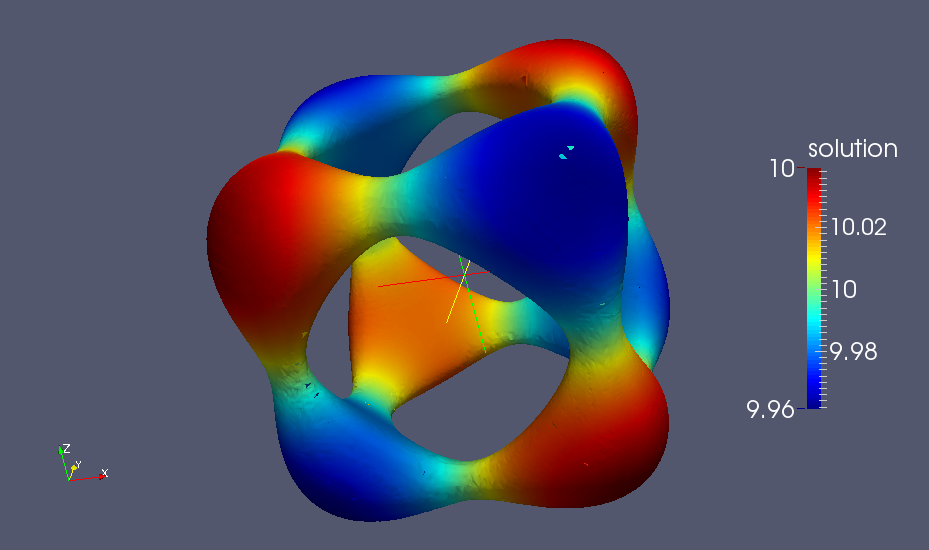
\includegraphics[width=0.7\textwidth]{example_newtorus.png}
			\end{figure}
\end{frame}
\begin{frame}{References}
	\begin{itemize}
		\item{S. Gross and A. Reusken: Numerical Methods for Two-phase Incompressible Flows, Springer 2011}
		\item{C. Lehrenfeld: Extenden finite element methods for interface problems, lecture notes, TU Wien 2015}
	\end{itemize}
\end{frame}

\end{document}